\chapter{二类问题实验评估}\label{sec:experiments}
\section{前言}
在第\ref{sec:method}章中,本文详细介绍了所提出模型的结构、背后的原理、损失函数等内容。接下来,本文将进行相关实验评估。实验评估分为第\ref{sec:experiments}章和第\ref{sec:multi_classes}章共两章内容展开介绍。{\color{red}{TODO}}
\section{数据集介绍}
在本章中,本文将详细介绍本文提出的模型在处理二类问题时的性能表现。在\ref{sec:usually_ds_intro}小节中,本文介绍了包括眼底病变数据集和黑色素瘤皮肤病病变数据集在内的诸多可用于生物标记物定位任务的常见数据集。考虑到本文的研究内容是生物标记物分布比较分散、生物标记物尺寸大小不一的生物标记物定位任务(黑色素瘤皮肤病病变图像中的异常区域所占比例通常在$1/3$以上且往往没有专门的正常图像),本文将使用包括二类视网膜糖尿病性病变数据集(\ref{subsec:bin_dr_ds}小节)和二类模拟皮肤病病变数据集(\ref{subsec:bin_simulated_skin_ds}小节)在内的两个数据集来评估我们提出的模型用于生物标记物定位的表现。因此,在实验评估之前非常有必要先详细介绍以上两个数据集,以便让读者对于本文要解决的问题能有更为清晰的认识与更为明了的理解。下面将进行相关内容的具体叙述。
\subsection{二类视网膜糖尿病性病变数据集}\label{subsec:bin_dr_ds}
二类视网膜糖尿病性病变数据集是来自Kaggle视网膜糖尿病性病变数据集(原始数据集的相关内容介绍请参见\ref{subsec:original_dr_dataset_intro}小节,在此不做赘述),该数据集由从Kaggle视网膜糖尿病性病变数据集中选择出来的2,101张包含明确的糖尿病生物标志物的异常图像和2,101张正常图像组成。同时,在预处理阶段,我们先将图像中没有信息的四个黑角去掉;另外,由于眼底图像中的视网膜基本是呈圆形的,故在此基础上,我们还提取了视网膜的边界再根据视网膜边界取其最大内接矩形,从而彻底去掉眼底图像中的不包含任何信息的黑色部分,最后将图像尺寸大小重新调整到$128\times 128$。来自二类视网膜糖尿病性病变数据集的部分图像举例如图\ref{subfig:bin_dr_ds_example}所示。另外,可通过比较图\ref{fig:biomarker_localization_example}与图\ref{subfig:bin_dr_ds_example},来对比视网膜糖尿病性病变图像预处理前后的差异。另外,一方面,为了在后续章节中说明本文模型方法的有效性以及增加实验结果的可信度;另外一方面,Kaggle视网膜糖尿病性病变数据集本身没有像素级标注而在所有的异常图像中标出所有生物标记物的精确位置又是极其昂贵的,因此,我们随机选出了40张眼底图像并请两位专业眼科医师对其中所有的生物标记物进行了像素级标注,用于后续章节的定量分析。

从图\ref{subfig:bin_dr_ds_example}可以看出,眼底图像中含有丰富的血管,呈现一种随机走向,并且包含非常丰富的毛细血管网,这种充分而又精细的血管纹理细节本身就给图像的重建增加了困难,而图像重建只是本文模型方法中最为基础的一步。我们注意到视网膜糖尿病性病变图像中的血管所在像素位置的梯度明显高于周围像素,为了让编码器-解码器重建图像更为容易,本文使用Sobel梯度算子~\cite{sobel2014history}沿着水平和竖直两个方向的提取图像每个像素的梯度,将其作为L1损失函数的权重。另外,图像之间的背景亮度不易,比如,图\ref{subfig:bin_dr_ds_example}中,第一行第三列图像背景较亮,而第二列第一行图像背景较暗。就生物标记物本身来说,也呈现一种分散、大小不一、不够明显而又难以被察觉的特点,而且还能发现,生物标记物本身的颜色与背景颜色比较相近,比如图\ref{subfig:bin_dr_ds_example}中的第二列第三行和第一列第三行图像,因此这些生物标记物很容易与背景相混淆,这也是在二类视网膜糖尿病性病变数据集上完成生物标记物精确定位任务最大的难点。二类视网膜糖尿病性病变图像的这些特点都表明在该数据集上完成生物标记物定位的任务极具挑战性。另外,视网膜糖尿病性病变也是当今导致病人失明的主要原因,说明了该任务的具有较大现实意义和应用潜能。注意,有些生物标记物的边界不仅呈现一种不规则状况,边界还十分模糊,用矩形框圈出生物标记物的位置相对比较容易,但是做出像素级精确标注却比较难,这也是本文只随机选出40张图像做标注的主要原因。

\subsection{二类模拟皮肤病病变数据集}\label{subsec:bin_simulated_skin_ds}
二类模拟皮肤病病变数据集包含带有人工生物标记的皮肤图像。为了生成这个数据集,我们首先从一个皮肤镜图像数据集~\cite{codella2018skin}(原始数据集相关内容介绍可参见\ref{subsec:original_dermatoscope_ds_intro}小节)中提取了2,920张图像尺寸大小为$128\times128$的正常图像(实际上是通过滑动窗口方式得到的图像区域块)。为了模拟真实皮肤图像中生物标志物的数量、大小和所在位置的随机变化,我们通过随机参数控制,在每个模拟皮肤图像的一定范围内随机生成这些参数的值。更具体地说,对于每张异常图像,从Image-Net数据集~\cite{deng2009imagenet}中随机选择一到三张图像,并将其调整为尺寸大小为$4\times 4$、$8\times 8$或$16\times 16$的缩略图。再将缩略图嵌入到皮肤图像中,最后将其局部平滑作为人工生物标记。最终,二类模拟皮肤病病变数据集中共有异常图像1310张,正常图像1460张。注意,此数据集中的所有异常图像的人工生物标记物都有像素级的标注。

从图\ref{subfig:bin_simulate_skin_example}中可以看出,二类模拟皮肤病病变数据集中图像之间的背景差异比较大,主要表现在颜色和亮度,比如图中第二行第三列图像背景为红色,较亮,而第一行第二列图像背景则较暗。注意,由于本文对于所有异常图像中的生物标记物都做了局部平滑处理,故此数据集中的生物标记物也显得比较真实,最为明显的特点是其边界比较模糊。再加上引入了生物标记物大小、数量和位置这三个随机变化量,这也大大增加了在此数据集上实现生物标记物的精确定位的难度。与二类视网膜糖尿病性病变数据集相比,虽然生物标记物在纹理结构上并没有前者复杂,但是二类模拟皮肤病病变数据集的优势在于拥有所有生物标记物的像素级标注,故可在整个数据集上进行全面的定性分析,来反应出各个模型方法在生物标记物精确定位任务上的性能表现,而二类模拟皮肤病病变数据集本身的模拟生物标记物也比较接近真实,从而保证了从该数据集得出的实验结果的可行性和可靠性,这也是设置该数据集的意义所在。
\begin{figure}[h!]
	\centering
	\begin{subfigure}{0.48\textwidth}
		\centering
		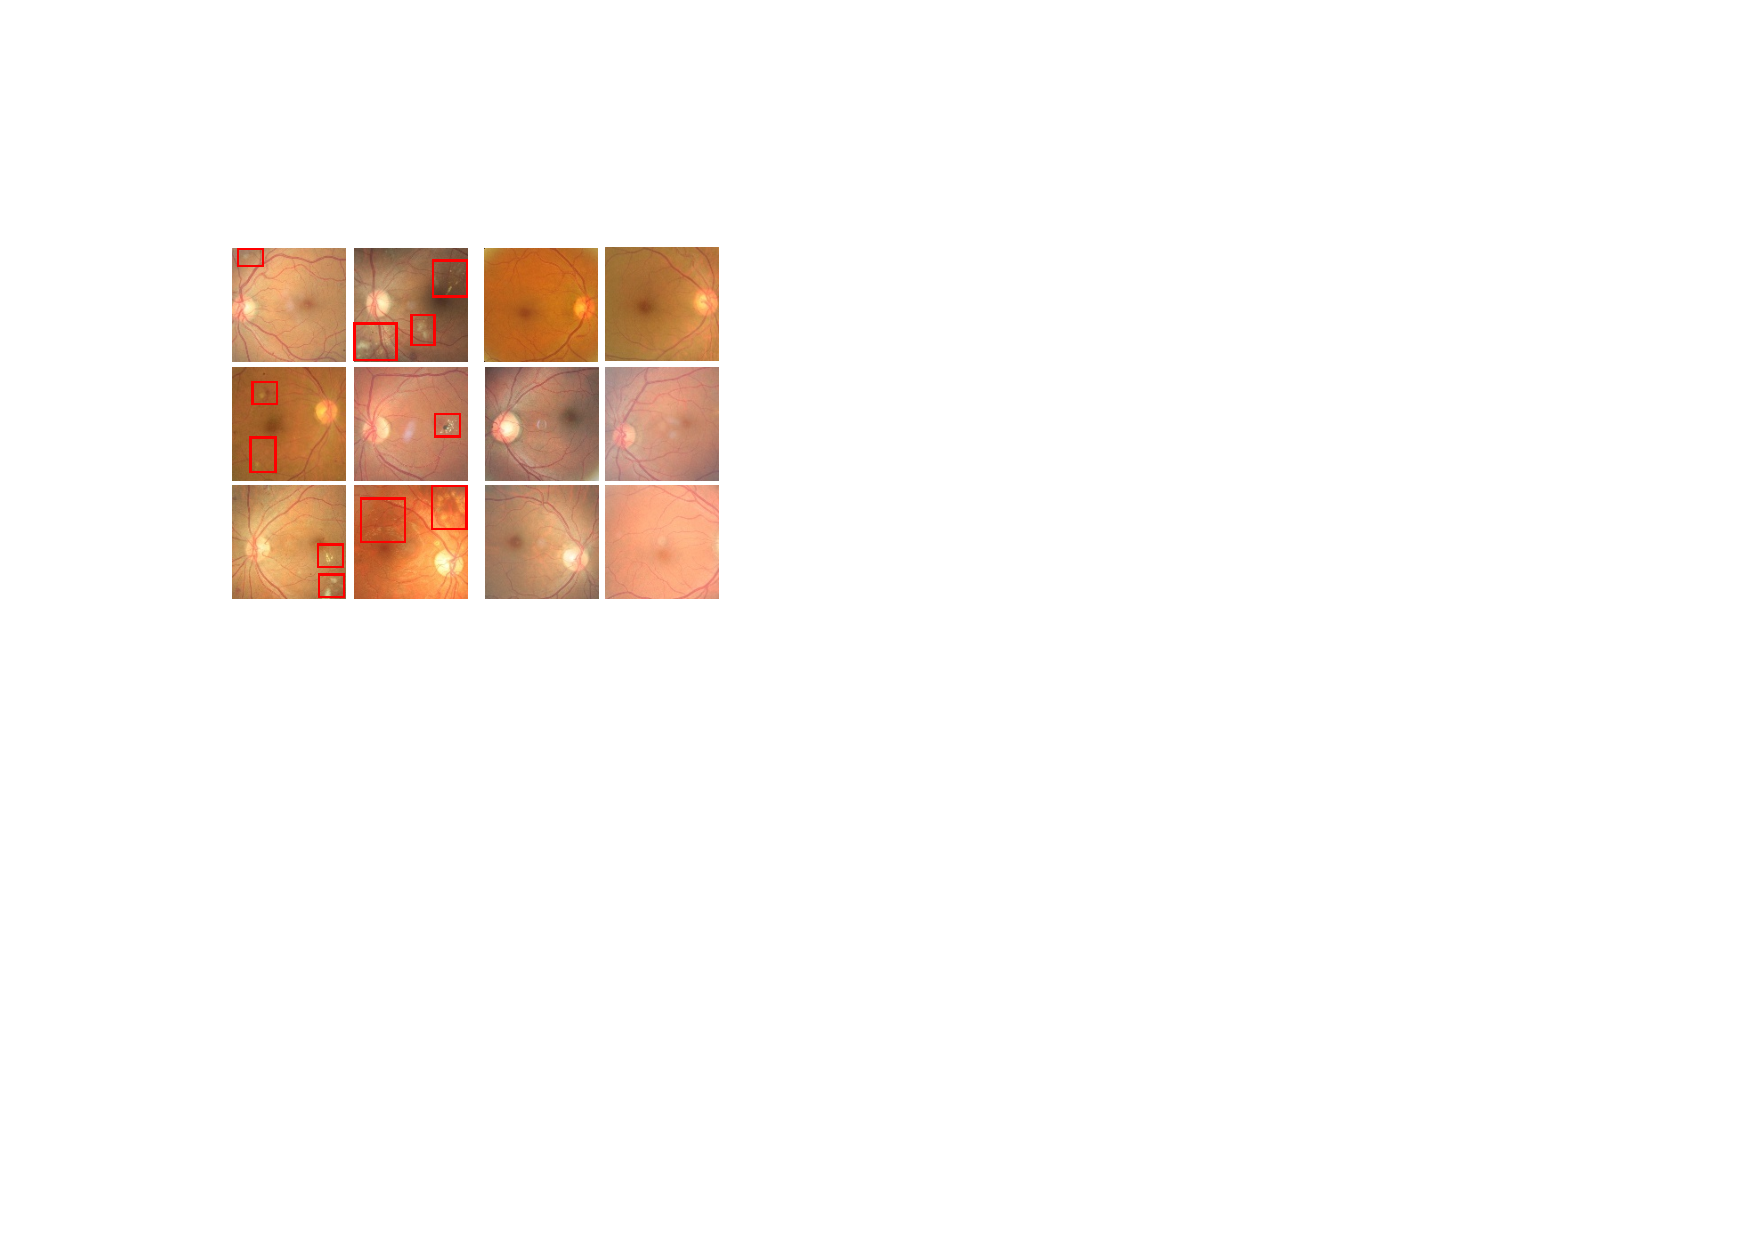
\includegraphics[width=1\textwidth]{figure/bin_dr_ds_example}
		\caption{二类视网膜糖尿病性病变数据集部分图像示例。第1、2列是异常图像,第3、4列是正常图像。}
		\label{subfig:bin_dr_ds_example}
	\end{subfigure}
	\quad
	\begin{subfigure}{0.48\textwidth}
		\centering
		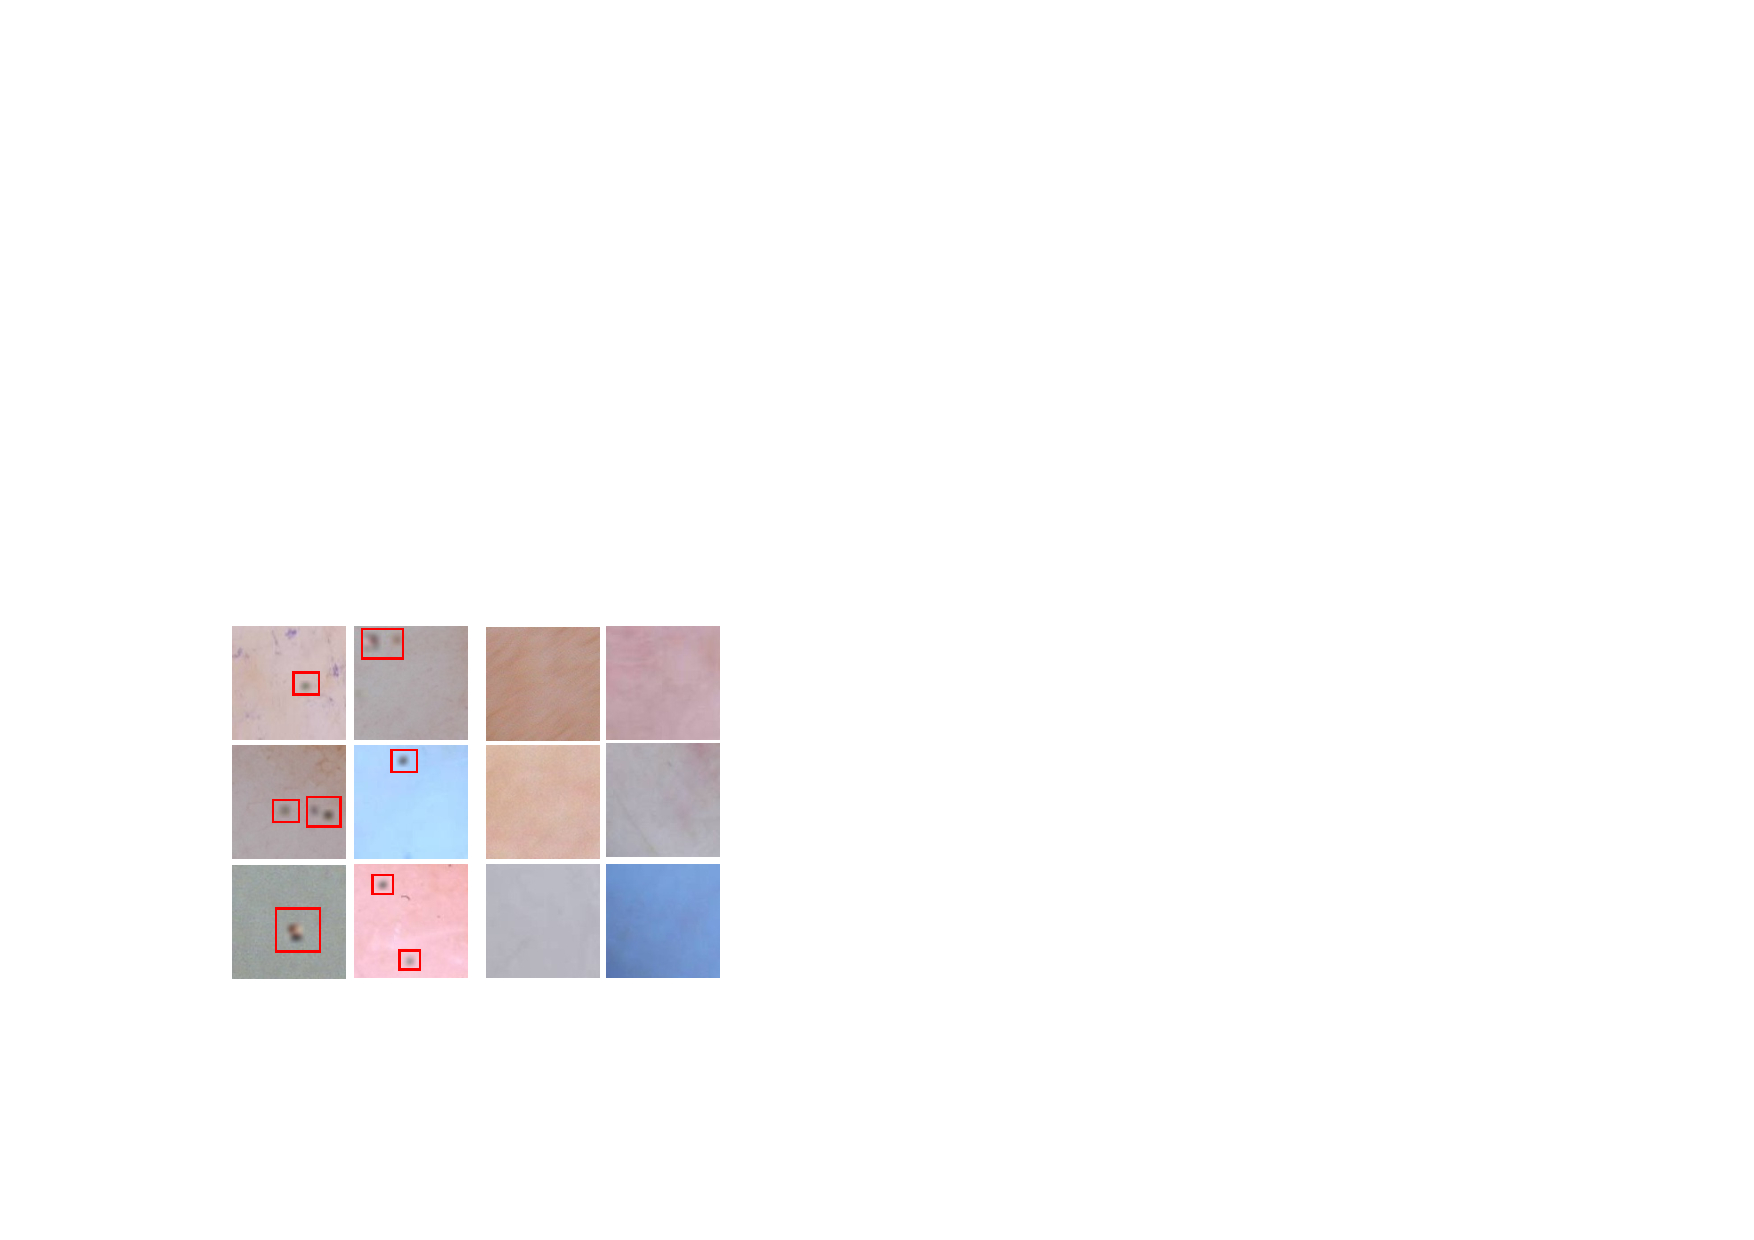
\includegraphics[width=1\textwidth]{figure/bin_simulate_skin_example}
		\caption{二类模拟皮肤病病变数据集部分图像示例。第1、2列是异常图像,第3、4列是正常图像。}
		\label{subfig:bin_simulate_skin_example}
	\end{subfigure}
	\caption{来自二类视网膜糖尿病性病变数据集和二类模拟皮肤病病变数据集的部分图像示例。红色矩形框表示框内存在生物标记物或者说框出区域是患病区域。在子图\ref{subfig:bin_dr_ds_example}中,每张图像中明显比周围要亮的圆形区域为视盘,为眼底图像的共有结构,而有些图像视盘在左边,有些视盘在右边,这是因为有些图像是左眼眼底图像,而有些是右眼眼底图像。}
	\label{mul_fig:bin_ds_example}
\end{figure}
\section{评价标准}
在\ref{subsec:roc_curve}小节和\ref{subsec:pr_curve}小节中,本文分别介绍了ROC曲线及其AUC和P-R曲线及其AUC,并在此过程中定义了FPR、TPR等相关概念。本文还在\ref{subsec:pr_curve}小节中说明了ROC曲线对正负样本分布的变化表现比较稳定,而P-R曲线在此情况下则更为敏感,故P-R曲线更能反映出在正负样本比例悬殊较大情况下系统的真实性能。

\begin{table}[h]
	\centering
	\caption{二类视网膜糖尿病性病变数据集和二类模拟皮肤病病变数据集图像像素数量统计表。}
	\label{tab:bin_ds_pixel_freqs}
	\begin{tabular}{c|c|c|c}
		\toprule[2pt]
		数据集名称 & 正常像素数量 & 异常像素数量 & 比例 \\
		\midrule[2pt]
		二类视网膜糖尿病性病变数据集&  $643,837$ & $11,523$ & $\simeq 56: 1$ \\ \hline
		二类模拟皮肤病病变数据集 & $21,222,487$ & $240,553$ & $\simeq 88: 1$ \\
		\bottomrule[2pt]
	\end{tabular}
\end{table}

\noindent 从表\ref{tab:bin_ds_pixel_freqs}可以看出,无论是二类视网膜糖尿病性病变数据集还是二类模拟皮肤病病变数据集,异常像素(正样本)和正常像素数量(负样本)之间的比例存在巨大悬殊甚至达到$88:1$。故接下来的实验部分均采用P-R曲线及其AUC作为主要评价标准,但是ROC曲线也会在本文附录\ref{chapter:append1}中进行展示,从而使得实验评估更为全面,对相关内容感兴趣的读者可自行查看。
\section{实验设置}
在提出的结构中,编码器-解码器网络选择一个经过修改的U-Net~\cite{iglovikov2018ternausnet},并在最后一层加入Tanh激活函数,将UNet输出的像素值约束在与UNet输入相同的范围内:[-1,1](更为详细的相关内容介绍可参见\ref{subsec:encoder_decoder_model}小节)。U-Net使用每个数据集的所有图像进行预训练。CNN分类器网络使用了一个Resnet-18, 判别器网络使用了一个$7$层卷积神经网络($4$个DownConv2d模块+$3$个Conv2dBlock模块,参见图\ref{fig:discrimintor_architecture})。WGAN-GP中的梯度惩罚系数$\lambda$损失被设置为10(与WGAN-GP原文中一致)。模型训练使用Adam优化器~\cite{kingma2014adam},默认学习率取$0.0002$,训练每次迭代取32张图像。对于所有的测试,$\lambda_1 = 0.4$和$\lambda_{2} = 10.0$。我们使用PR曲线进行定量评估,它是通过比较像素级定位结果和真实二值标签(1表示生物标记物,0表示正常)得到的。在生成P-R曲线之前,定位结果的热图被归一化为$[0,1]$。请注意,ROC曲线并不适合用来评价生物标记物的定位性能,因为每个数据集的正、负像素的比例非常不平衡(参考表$\ref{tab:bin_ds_pixel_freqs}$)。因此,本文正文中只展示相关实验的P-R曲线。

请注意,我们的目标是通过图像级标签从已有图像中搜索和定位生物生物标记(像素级),而不是训练模型从新图像中寻找生物标记物。因此,对于每个数据集,所有的图像都被用来训练我们的模型,然后对模型进行定性和定量的评估。因此,我们将在相同的数据集上训练和评估我们的模型。

\section{在二类视网膜糖尿病性病变数据集上的实验结果分析}\label{sec:bin_dr_ds_experiment}
本节将展示本文提出的模型在视网膜糖尿病性病变数据集上的实验结果,本文提出的模型将与CAM和Grad-CAM共计两种用于卷积神经网络的可视化方法作定性分析和定量分析。下面展开相关内容的具体阐述。

CAM和Grad-CAM最为一种用于CNN可视化的方法,本身需要分两步完成。需要先训练得到一个分类器,再通过特征图的可视化来间接完成生物标记物的定位。一方面为了尽量减少与实验内容无关的因素干扰,另一方面由于CAM只能完成对最后一层是全局均值池化层的卷积神经网络的可视化(相关解释可参见\ref{subsec:gradient_based_methods}小节),综合以上因素,本文将ResNet-18作为CAM和Grad-CAM可视化的目标CNN分类器。另外,为了排除由于CNN性能的缺陷导致可视化结果表现较差,本文同样使用数据集中的所有图像来训练ResNet-18分类器,即没有为ResNet-18单独设置测试集,本文后续所有关于CAM和Grad-CAM的相关实验结果均在此条件设置下完成。在使用视网膜糖尿病性病变数据集训练ResNet-18时,分类器最终的分类准确率达到了100\%。由于Grad-CAM可对任意层输出的特征图完成可视化,从而实现生物标记物的定位。因此,如图\ref{fig:retinal_image_res}所示,本文展示出了使用Grad-CAM对中间层特征输出(第$4$列)和最后一层特征输出(第$5$列)的生物标记物定位结果(可与CAM作比较)。
\begin{figure}[h]
	\centering
	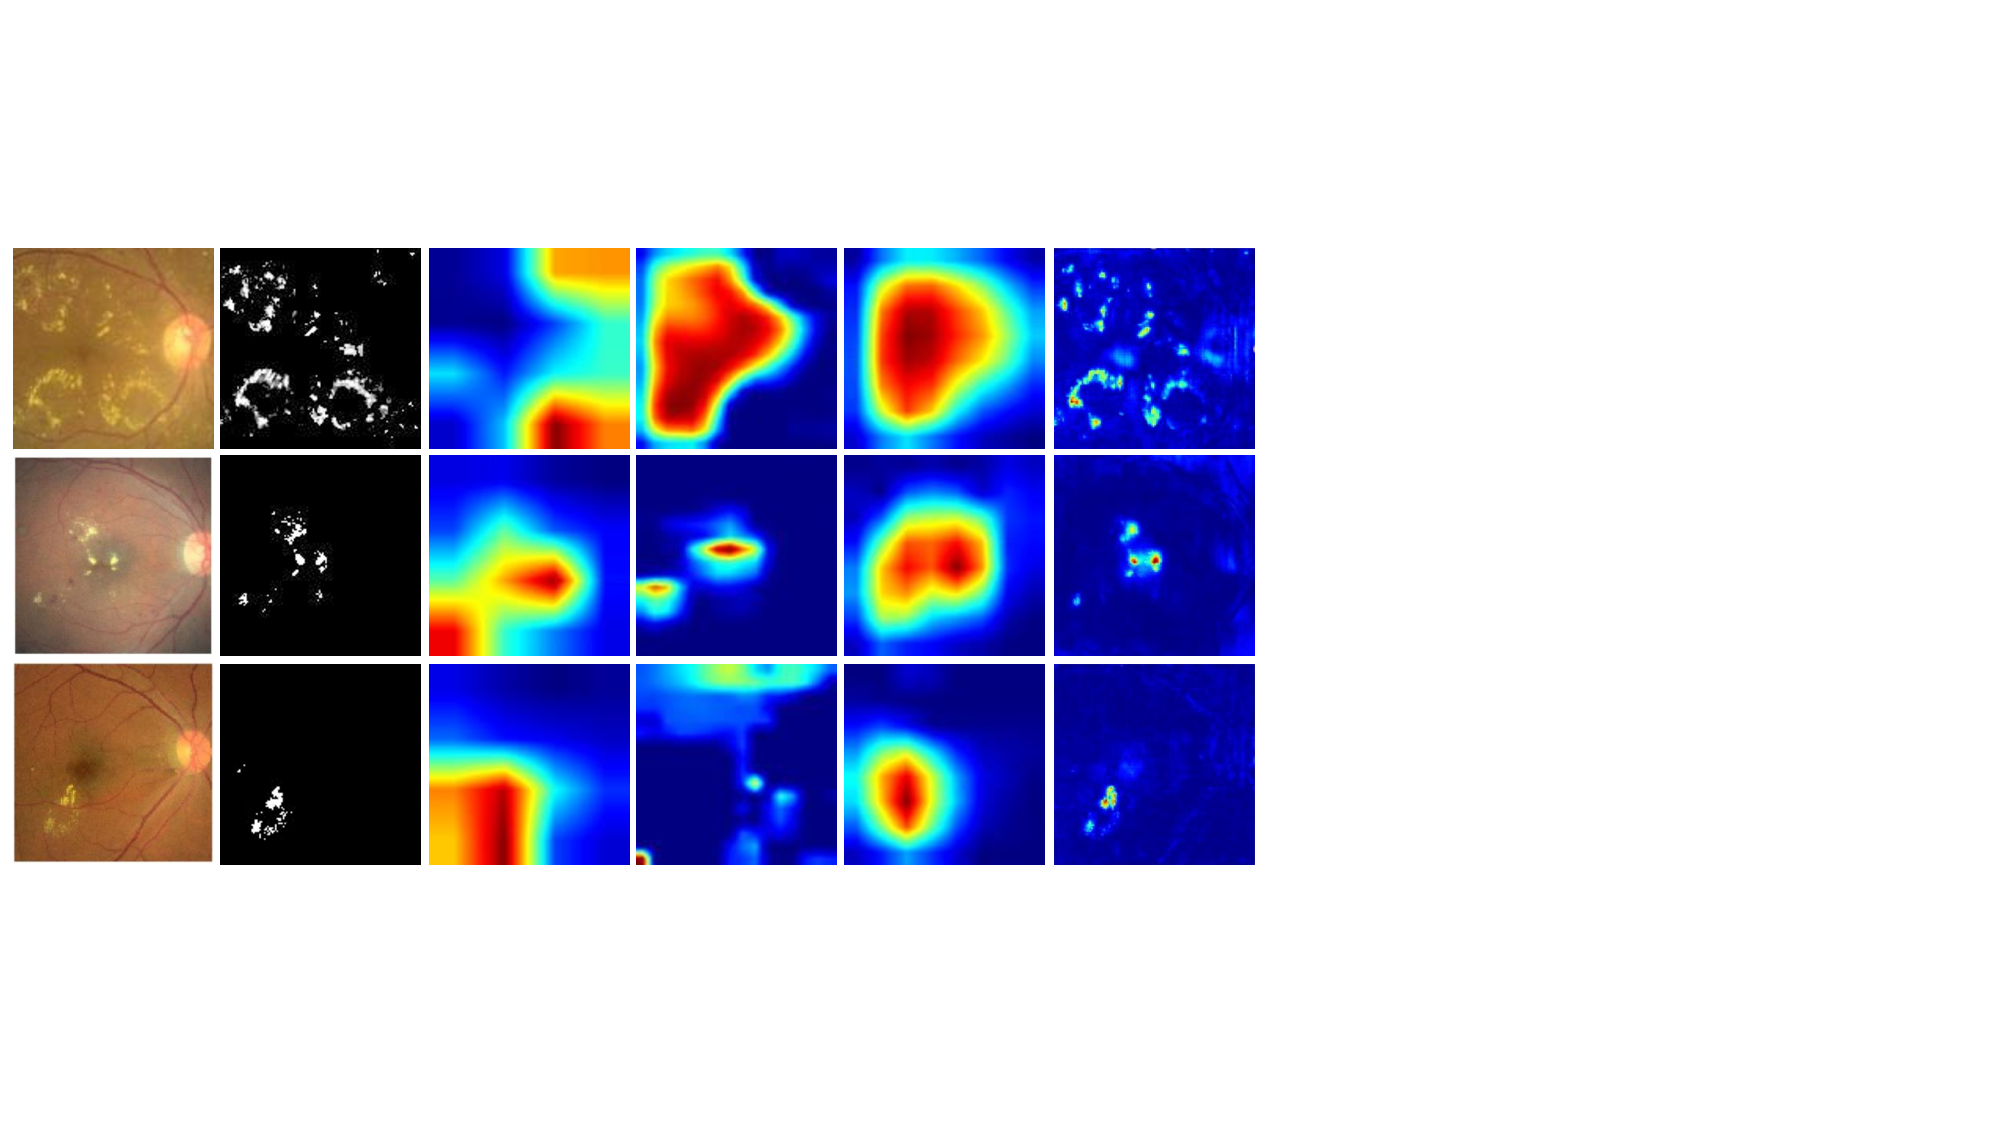
\includegraphics[width=1.0\textwidth]{figure/retinal_image_res.pdf}
	\caption{在视网膜糖尿病性病变数据集上生物标记物定位结果。图中第$1$列表示原始异常图像,第$2$列表示其像素级标注,第$3$列表示CAM的定位结果,第$4$列表示Grad-CAM使用分类器中间层的特征图可视化的定位结果,第$5$列表示Grad-CAM使用分类器最后一层特征图可视化的定位结果,第$6$列是本文提出模型的定位结果。}
	\label{fig:retinal_image_res}
\end{figure}

\noindent 如图\ref{fig:retinal_image_res}所示,从图中第$3$列定位结果可以看出,虽然CAM发现的生物标记物或者说异常区域最多,但是CAM也将周边区域作为生物标记物的一部分。这主要是由于将最后一个卷积层($4\times 4$)的输出向上采样到图像大小($128\times 128$)。另外,CAM也未能检测到第一幅图像(第$3$列,第$1$行)中的大部分异常区域。Grad-CAM作为CAM的扩展,它允许我们从多个层生成可视化的解释,例如中间卷积层(第$4$列,可记为Grad-CAM-1)和最后卷积层(第$5$列,可记为Grad-CAM-2)。虽然Grad-CAM-1在第$4$列(第三幅图像)获得了较为准确的生物标记物定位结果,但通过也将正常区域(图像中中间上方区域和左下角区域)误认作包含生物标记物的异常区域。更多的是其结果要么不够精确(第$1$行),要么不够精确(第$2$行和第$3$行)。与CAM相比,Grad-CAM-1实现了更为精确的定位结果,证明了其优于CAM的性能。另外,同样是由于对可视化特征图悬殊的上采样倍数($4\times 4 \rightarrow 128\times 128$),可以发现,Grad-CAM-2(第$5$列)标记的区域和CAM(第$3$列)没有太大区别。相比直线,本文提出的方法对形状不规则、分布分散的生物标记物进行了更精确的局部化(第$6$列),从定性分析的角度证明了其优于CAM和Grad-CAM的性能。

另外,本文充分利用视网膜糖尿病性病变数据集中的$40$张像素级标注,通过对每种方法的定量评价,本文提出的模型、CAM、Grad-CAM-1和Grad-CAM-2的P-R曲线如图\ref{fig:retinal_image_pr_curve}所示。以上四种方法各自对应的P-R曲线下的面积(AUC)分别为$0.481$,$0.065$,$0.061$和$0.042$,从而进一步从定量分析的角度证明了本文提出的模型的性能优越性。

\begin{figure}[h]
	\centering
	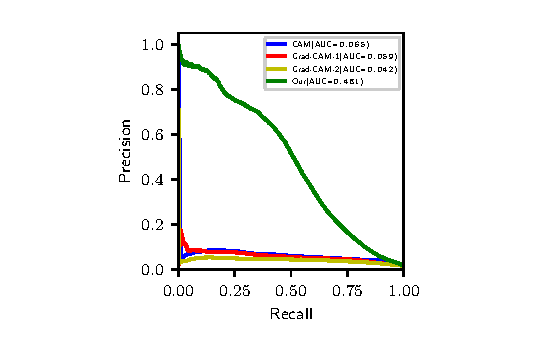
\includegraphics[width=1.0\textwidth]{figure/pr_curve_retinal_image/pr_curve.eps}
	\caption{本文提出的模型、CAM、Grad-CAM-1和Grad-CAM-2在40张视网膜糖尿病性病变图像上画出的P-R曲线及其各自曲线下的面积(AUC,见右上角图例)。} 
	\label{fig:retinal_image_pr_curve}
\end{figure}

\section{在二类模拟皮肤病病变数据集上的实验结果分析}
本节将展示本文提出的模型在模拟皮肤病病变数据集上的实验结果分析,本文提出的模型的比较对象同样是与CAM和Grad-CAM共计两种用于卷积神经网络可视化的方法进行比较,分定量分析和定性分析两个角度展开,下面进行具体叙述。

与\ref{sec:bin_dr_ds_experiment}小节一样,在本实验中,依然将ResNet-18作为CAM和Grad-CAM可视化的目标CNN分类器,同样没有单独设置测试集,分类器最终CNN分类准确率均达到了$99.7\%$以上。类似的,由于Grad-CAM可对卷积神经网络的任意层输出特征进行可视化,故在此实验中,同样选择了中间层输出特征(见图\ref{fig:simulated_skin}第$4$列)和最后一层输出特征(见图\ref{fig:simulated_skin}第$4$列)进行可视化,从而定位生物标记物。
\begin{figure}[h]
	\centering
	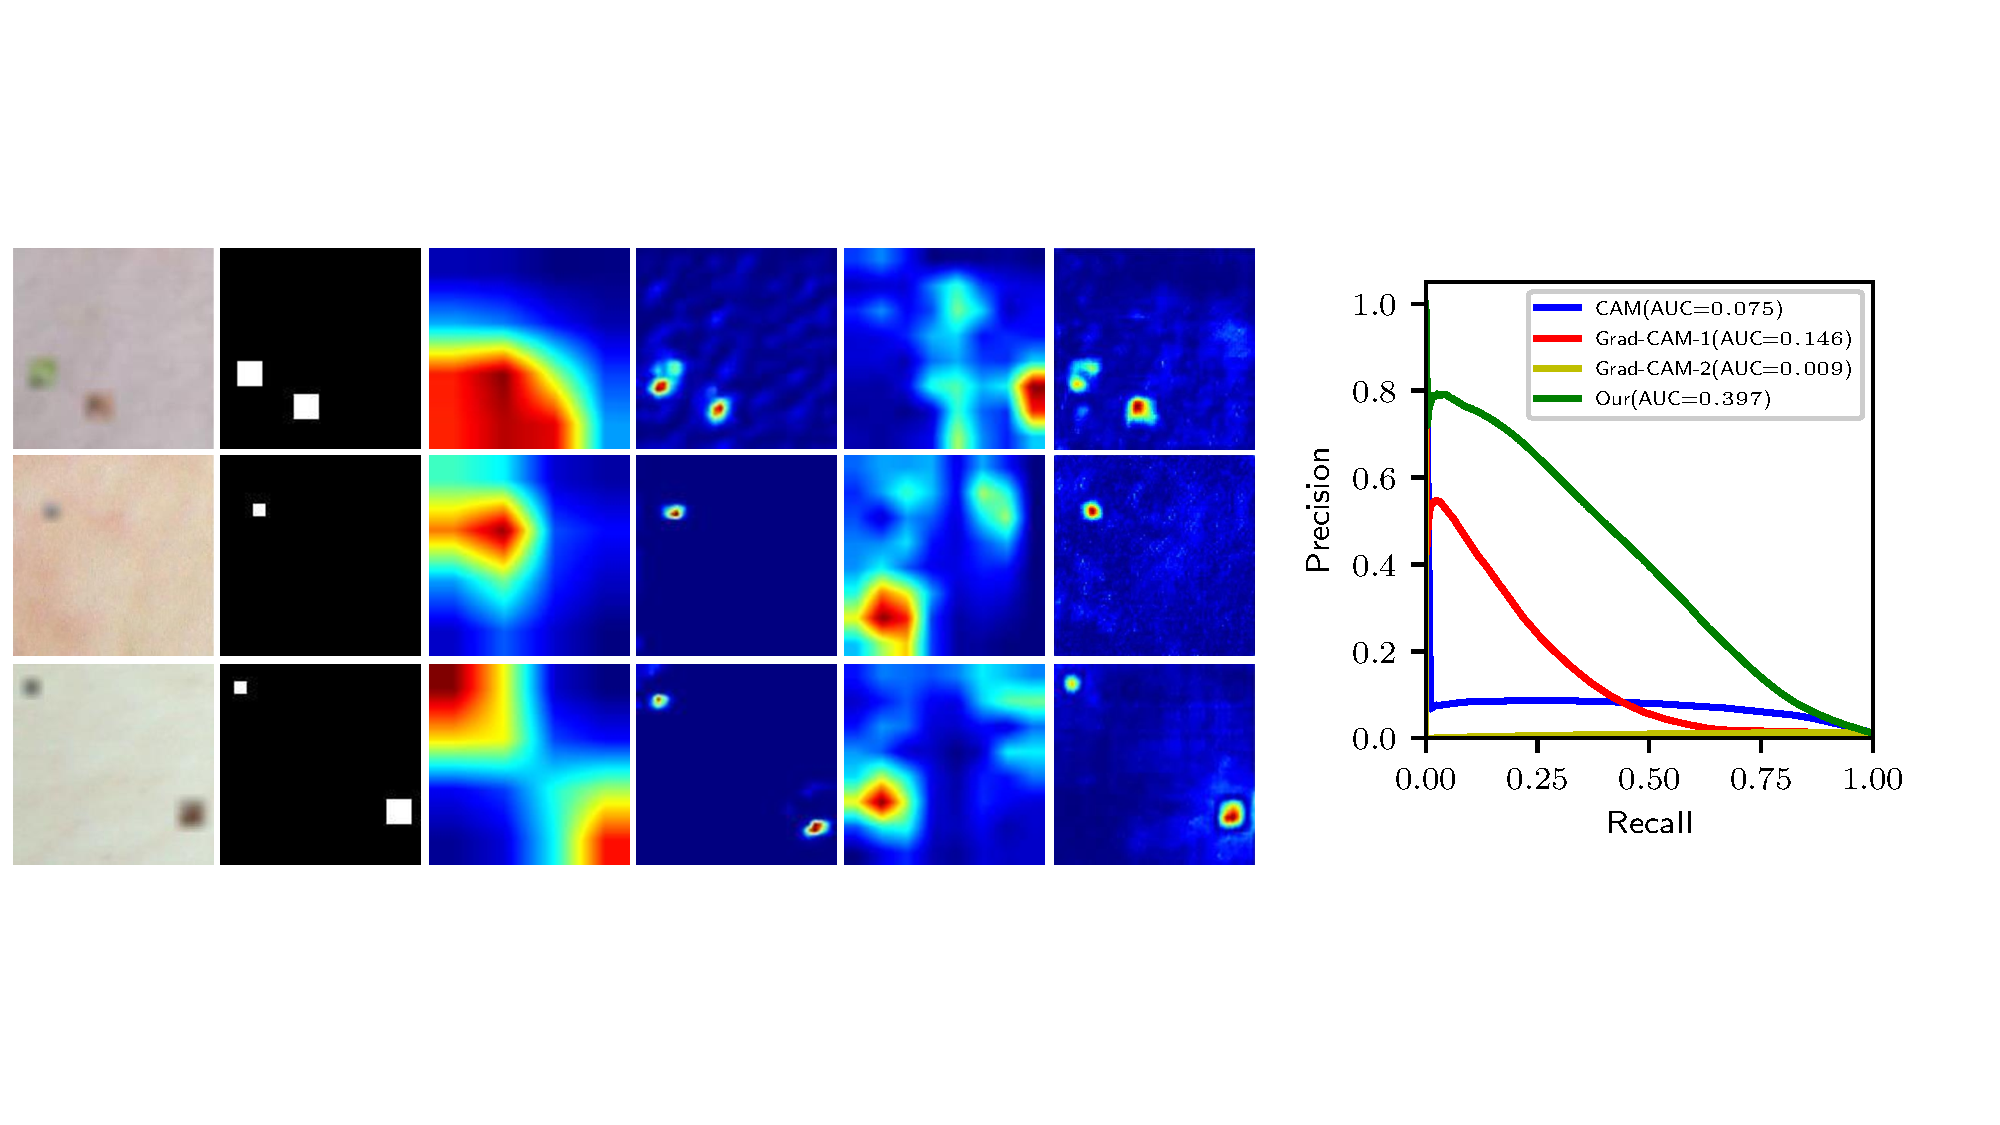
\includegraphics[width=1.0\textwidth]{figure/pr_curve_skin_image.pdf}
	\caption{在二类模拟皮肤病病变数据集上的生物标记物定位结果。图中第$1$列表示原始异常图像,第$2$列表示其像素级标注,第$3$列表示CAM的定位结果,第$4$列表示Grad-CAM使用分类器中间层的特征图可视化的定位结果(Grad-CAM-1),第$5$列表示Grad-CAM使用分类器最后一层特征图可视化的定位结果(Grad-CAM-2),第$6$列是本文提出模型的定位结果。} 
	\label{fig:simulated_skin}
\end{figure}

\noindent 从图\ref{fig:simulated_skin}可以看出,人工模拟生物标志物的皮肤图像进一步证实了本文提出的模型的优越性能。从图\ref{fig:simulated_skin}第$6$列可以看出,本文提出的方法几乎可以完美、精确地定位人工生物标记物,而CAM(第$3$列)和Grad-CAM(第$4$列和第$5$列)的性能再次表现出劣势。从总体上来说,第$4$列中生物标记物定位结果明显要比第$3$列更精确、更完美,也就能说明Grad-CAM在定位生物标记物上优于CAM。同样是由于特征图的过度上采样,CAM(第$3$列)和Grad-CAM-2(第$5$列)呈现类似的定位结果:虽然能检测到生物标记物的位置,但同时也包含了生物标记物周围的大量正常像素。之所以Grad-CAM-1(第$4$列)基本能精确定位到生物标记物的位置而极少包含生物标记物的周围像素,主要是因为Grad-CAM-1是通过对ResNet-18中第一个卷积层的特征输出的可视化结果来完成生物标记物的定位,其中上采样倍数较小($64\times 64\rightarrow 128\times 128$),这也能从侧面说明在该数据集上定位生物标记物要比在二类视网膜糖尿病性病变数据集上容易得多(浅层特征便具备高级语义)。而CAM和Grad-CAM-2却都选择了最后一层卷积层的输出特征,其中上采样倍数要大得多($4\times4\rightarrow 128\times 128$)。

图5(右)证实了我们的模型(AUC=0.397)优于CAM (AUC=0.075)、graden -CAM-1 (AUC=0.146)和graden -CAM-2 (AUC=0.009)。


\begin{figure}[h]
	\centering
	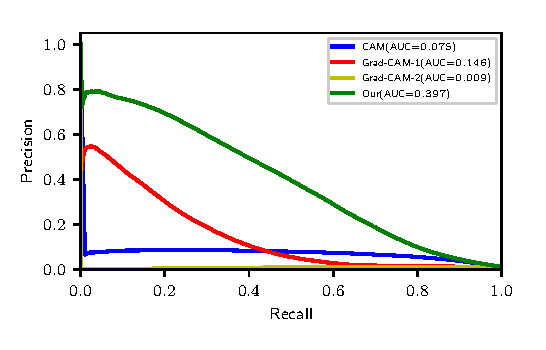
\includegraphics[width=1.0\textwidth]{figure/pr_curve_skin_image/pr_curve.eps}
	\caption{}
	\label{fig:simulated_skin_pr_curve}
\end{figure}

\section{消融实验:生成器和判别器角色探究}
\begin{figure}[h]
	\centering
	\includegraphics[width=1.0\textwidth]{figure/u_d_c_comparation.pdf}
	\caption{} 
	\label{fig:u_d_c_comparation}
\end{figure}
\begin{figure}[h]
	\centering
	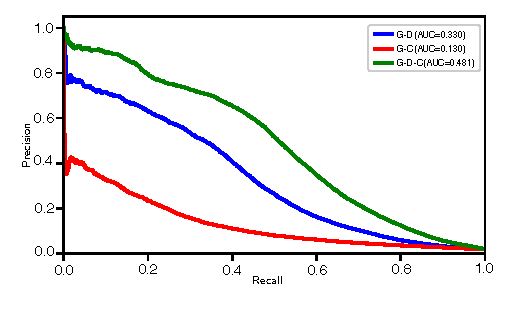
\includegraphics[width=1.0\textwidth]{figure/pr_cureve_u_d_u_c_u_d_c_components.pdf}
	\caption{} 
	\label{fig:u_d_c_comparation_pr_curve}
\end{figure}

\section{本章小结}



